En este capítulo se describe la metodología propuesta para el descubrimiento de tópicos y su evolución en el tiempo. En primer lugar, en la sección \ref{sec:processing} se describe la metodología de procesamiento utilizada para limpiar los datos que usa el modelo. En segundo lugar, en la sección \ref{sec:model_selected} se justifica la elección del modelo de tópicos. En tercer lugar, en la sección \ref{sec:build_graph} se describe la metodología escogida para modelar la evolución en el tiempo y la médida de similitud utilizada para comparar tópicos de épocas adyacentes. En cuarto lugar, en la sección \ref{sec:hiperparameters} se describen los hiperparámetros y su configuración. Por último, en la sección \ref{sec:methodology_resume} se resume de manera global la metodología.

\section{Procesamiento}
\label{sec:processing}

El propósito del procesamiento es simplificar eliminar el ruido en los datos y a su vez mantener el \textit{core} de palabras del corpus. En el caso del modelamiento de tópicos, esta etapa puede reducir significativamente el vocabulario. Como consecuencia, esto puede traer una mejora en la significancia estadística de los modelos, puesto que se puede obtener un mejor balance entre cantidad de parámetros y observaciones. Adicionalmente, puede facilitar la interpretación de los tópicos, removiendo palabras que aportan poca información.\\

En este experimento se aplicaron las siguientes cinco etapas:
\begin{enumerate}
  \item \textbf{Tokenización}: La tokenización es una operación sobre una cadena de caracteres (\textit{string}) que consiste en dividir el \textit{string} en un conjunto de términos (ej: en base al caracter espacio), obteniéndose así una lista de elementos llamados \textit{tokens}, que en términos simples pueden considerarse como palabras.
\item \textbf{Procesamiento de caracteres}: En esta etapa se suelen aplicar algunas operaciones básicas de procesamiento. En este proceso se llevan los tokens a unicode y minúsculas. Luego, se eliminan patrones de caracteres que difícilmente pueden tener algún significado, como correos electrónicos, símbolos de puntuación, tokens con números y letras o solo números. 
\item \textbf{Eliminación de stopwords}: Las \textit{stopwords} \citep{wilbur1992automatic} son palabras que aportan poca información (ej: artículos, preposiciones y conectores), usualmente tienen un alta frecuencia dentro del corpus. Para esto se utiliza una lista de palabras disponibles en el paquete NLTK de Python, el cual contiene 313 palabras \citep{bird2009natural}. Además, esta lista es alimentada con 951 \textit{stopwords} contextuales que corresponden a palabras específicas del corpus que aportan poca información. En el caso del robo de vehículos palabras relacionas a \quotes{robo} o \quotes{vehículo} no aportan ninguna información, puesto a que todos los relatos hablan del robo de un vehículo. 
\item \textbf{Filtro por vocabulario}: Con el propósito de mantener palabras \quotes{humanamente legibles} se utiliza un vocabulario. Para esto se utiliza el vocabulario del corpus SUC que se describe en la sección \ref{sec:word_embeddings}, de esta manera toda palabra tiene su \textit{word embedding}. 
\item \textbf{Filtro por frecuencia}: En este nivel se eliminan los \textit{tokens} con baja frecuencia, dado que un modelo difícilmente aprenderá algún patrón de un evento que tiene muy pocas realizaciones, menos si tiene una realización única. Esta etapa se aplica a nivel época, eliminando aquellos tokens que aparecen en menos del 0.1\% de los documentos de su respectiva época.
\item \textbf{Eliminación de documentos}: En el último nivel se eliminan aquellos documentos que presentan pocos tokens. Esto tiene por objetivo obtener estimaciones más confiables y reducir la posibilidad de sacar conclusiones prematuras debido a las pocas observaciones con las que cuenta un documento. En este caso se eliminan documentos que presentan menos de 5 tokens.
\end{enumerate}

\section{Modelos de tópicos}
\label{sec:model_selected}

Se escoge HDP como el modelo de tópicos base de la metodología. Si bien, HDP es un modelo similar en estructura a LDA, su principal ventaja es que el número de tópicos no está acotado y es inferido a partir de los datos, en cambio LDA requiere de escoger el número de tópicos $K$ por adelantado. \\

En un enfoque tradicional, se requiere de entrenar múltiples veces LDA para diferentes valores de $K$ y se escoge la configuración con mejor desempeño en un conjunto de validación, por lo que LDA termina siendo computacionalmente más costoso que HDP, además este enfoque se vuelve impracticable cuando el conjunto de datos es lo suficientemente grande. \\

En el aspecto cualitativo ambos modelos entregan tópicos igual de consistentes. En cuanto a métricas de desempeño como $\textit{perplexity}$ HDP suele tener mejor desempeño \citep{teh2005sharing}.\\

Para el descubrimiento de tópicos se utiliza la implementación disponible en C++ \citep{HDP} de HDP para modelamiento de tópicos. Esta implementación está basada en el algoritmo de Gibbs Sampling propuesto en \citep{teh2005sharing}.

\section{Construcción del grafo temporal}
\label{sec:build_graph}

El objetivo del trabajo no es solo descubrir tópicos sino también modelar sus interacciones en el tiempo, como nacimiento, muerte, evolución, divisón y fusión.
Así, la metodología propuesta se basa en la metodología descrita en la sección \ref{sec:similarity_graph}, debido que esta captura los dinamismos mencionados.\\

En general, las medidas de similitud o distancia comparan vectores con el mismo dominio y dimensión, esto significa que los tópicos de épocas adyacentes deben compartir el mismo vocabulario. Matemáticamente, sea $\phi_{t, i}$ un tópico de la época $t$ y $V_{t}$ su vocabulario, sea  $\phi_{t+1, j}$ un tópico de la época $t+1$ y $V_{t+1}$ su vocabulario. Con una alta probabilidad existen palabras en $V_{t}$ que no están en $V_{t+1}$ y viceversa. Para poder comparar tópicos en épocas adyacentes  es necesario contar con un vocabulario global $V_{t+1}^{'}=V_{t}\cup V_{t+1}$, luego aplicar $padding$ a los vectores $\phi_{t, i}$ y $\phi_{t+1, j}$, es decir, rellenar con ceros las posiciones que no están en el vocabulario de su dominio.\\

Una gran desventaja del enfoque anterior es que no captura similitud entre palabras, puesto que cada palabra ocupa una posición dentro del vector y no hay forma de comparar palabras que no son comúnes en ambas épocas. El peor caso sería considerar $V_{t}\cap V_{t+1} =  \emptyset$, a pesar de que cada palabra en $V_{t}$ tuviese un sinónimo en $V_{t+1}$ la similitud entre tópicos entre las épocas $t$ y $t+1$ sería cero.\\

\subsection{Word Mover's Distance}

Para lidiar con el problema anterior, se propone utilizar una medida de distancia conocida como Word Mover's Distance (WMD) \citep{kusner2015word}, medida utilizada para comparar dos documento bajo una representación \textit{bag of words} a través de sus \textit{word embeddings} \citep{mikolov2013distributed}.\\

WMD calcula el costo mínimo de transformar un documento en otro, en esto caso particular sería el costo mínimo de llevar un tópico a otro. Para esto se resuelve el problema de transporte, donde los flujos son los pesos $\phi_{t,i}$ y $\phi_{t+1,j}$ y la matriz de costos es una matriz de distancia euclidiana entre los \textit{word embedding} de todas las palabras de $V_{t}$ con $V_{t+1}$. En la Figura \ref{img:wmd_obama} se ilustra el espacio en el que viven las palabras de dos documentos.

\begin{figure}
    \centering
    \includegraphics[width=1\textwidth]{ch3/wmd-obama.png}
    \caption{Espacio vectorial de los \textit{word embeddings} de las palabras de dos documentos con un vocabulario de tamaño 4. Fuente: Figura de \citep{WMDPy}.}
    \label{img:wmd_obama}
\end{figure}

Sea  $V_{i}$ y $V_{j}$ los vocabularios del tópico $i$ y $j$ respectivamente, luego su WMD viene dado por $WMD(\phi_{i}, \phi_{j})$:

\begin{align}
\underset{x}{\text{min}}&\sum_{u \in V_{i}}\sum_{v \in V_{j}} c_{u,v}x_{u,v} \\ 
\textrm{s.t.} &\sum_{v \in V_{j}}x_{u,v}= \phi_{i,u}, \; u \in V_{i}\\ 
& \sum_{u \in V_{i}}x_{u,v}= \phi_{j,v}, \; v\in V_{j}\\
& x_{u,v} \geq 0,\; u \in V_{i} \;, v \in V_{j}\\ \nonumber
\end{align}

Donde $x_{u,v}$ es el flujo que va de la palabra $u$ del tópico $i$ a la palabra $v$ del tópico $j$, $\phi_{i,u}$ es la probabilidad de la palabra $u$ en el tópico $i$, $c_{u,v}$ es el costo de mover una unidad de flujo por el arco $(u,v)$, el costo entre palabras se mide como la distancia euclidiana entre los \textit{word embedding} de dichas palabras.\\

La primera restricción indica que el flujo que se mueve de una palabra $u$ del tópico $i$ a todas las palabras del tópico $j$ debe sumar su peso ($\phi_{i,u}$), la segunda restricción significa que el flujo que se mueve de una palabra $v$ del tópico $j$ a todas las palabras del tópico $i$ debe sumar su peso ($\phi_{j,v}$). Lo anterior implica que esta medida de distancia es simétrica, es decir, $WMD(\phi_{i}, \phi_{j}) = WMD(\phi_{j}, \phi_{i})$.\\

La WMD se puede transformar fácilmente en una médida de similitud considerando $\rho(\phi_{i}, \phi_{j}) = \frac{1}{1+WMD(\phi_{i}, \phi_{j})}$. Notar que si la WMD es 0 la similitud es 1 y si es $\infty$ la similitud es 0. \\

\subsection{WMD complejidad}
\label{sec:wmd_complexity}

WMD es una medida de distancia intensiva en recursos computacionales. Para ilustrar lo anterior se utiliza la representación poliedral del problema. Sea $N$ el tamaño del vocabulario entre dos épocas adyacentes, luego la región factible del problema anterior se puede representar como $\{x| Ax=b, x\geq 0\}$ sobre un grafo bipartito, con $A\in \mathbb{R}^{2N\times N^{2}}$ la matriz de incidencia, $b\in \mathbb{R}^{2N}$ la capacidad de los nodos y $x\in \mathbb{R}^{N^{2}}$ el flujo a enviar por cada uno de los arcos. La implementación utilizada es la de \citep{PyEMD}, la cual está basada en el algoritmo \citep{pele2009fast}, cuya complejidad del mejor tiempo promedio escala $\mathcal{O}(N^{2}log N)$.\\

Los tópicos siguen una distribución con forma de ley de potencia sobre el vocabulario, donde una pequeña fracción de las palabras concentran la mayor parte de la masa de la distribución. Además, en la práctica la interpretación de los tópicos se basa en los top $N$ palabras más probables, usualmente con $N \in [5, 30]$, entonces, se puede aprovechar esta estructura para efectos de computar la WMD de un forma más eficiente, por ejemplo, utilizando solo las palabras que capturan un determinado porcentaje de la distribución acumulada del tópico. Por ejemplo, si se reduce el vocabulario a un décimo en el peor caso promedio se obtiene un \textit{speed up} de 200.\\

\subsection{Word Embeddings}
\label{sec:word_embeddings}

Computar WMD requiere contar con \textit{word embeddings}. Para estó se escoge una de las más grandes colecciones de \textit{word embeddings} en español \citep{fastextSUC}, que cuenta con 1,313,423 \textit{embeddings}, colección obtenida utilizando el algoritmo FasText \citep{bojanowski2017enriching} sobre el corpus Spanish Unannotated Corpora (SUC) \citep{josecanneteSUC}, uno de los más grandes corpus de texto en español. FasText en comparación a otros enfoques para extraer \textit{embeddings} representa los \textit{tokens} a través de n-gramas de caracteres, de esta manera puede obtener \textit{embeddings} de \textit{tokens} no vistos durante el entrenamiento a partir de los \textit{embeddings} de los caracteres que lo componen.

\section{Configuración de hiperparámetros}
\label{sec:hiperparameters}

En la metodología propuesta se pueden considerar dos fuentes de evaluación de desempeño, el descubrimiento de tópicos y cómo se relacionan. En ambos casos no se cuenta con el \textit{ground truth} para medir correctamente el desempeño. Si se conociera el \textit{ground truth}, se podría utilizar la métrica \textit{purity} \citep{manning2008introduction} para comparar la asignación de los documentos en torno a los tópicos con la etiqueta. En el caso del grafo temporal, si se conocieran las conexiones presentes y ausentes se podrían utilizar métricas de clasificación.\\

\subsection{Configuración de hiperparámetros de HDP}
\label{sec:hdp_hiperparameters}

HDP cuenta con tres hiperparámertos, el parámetro de concentración a nivel corpus $\gamma$, el parámetro de concentración a nivel documento $\alpha_{0}$ y $\eta$ el parámetro de la medida base Dirichlet.\\

En \citep{blei2003latent,griffiths2004finding,cao2009density,arun2010finding,deveaud2014accurate,zhang2017lda} se describen algunas métricas que no requieren de una etiqueta, que pueden ser útil para realizar selección de modelo de tópico. Cabe destacar que estas métricas carecen de significado y sirven para comparar si un modelo de tópicos es superior a otro.\\

En general, en modelamiento de tópicos se prefiere usar $\eta\in (0,1)$, esto generará distribuciones \textit{sparse} sobre el vocabulario. Así, se suelen tener tópicos más distinguibles, donde el \textit{core} de palabras del tópico concentra la masa de la distribución. Además, como la semántica del tópico está compactada en pocas palabras se facilita la interpretación. En este caso se escoge un punto intermedio, fijando $\eta=0.5$.\\ 

En \citep{teh2005sharing} los parámetros de concentración se integran afuera usando un prior \textit{vague gamma} \citep{escobar1995bayesian}. Un prior \textit{vague gamma} es una distribución Gamma con una gran parte de la masa en torno a cero y una cola pesada. Véase la Figura \ref{img:gamma} para una ilustración de la pdf para diferentes parámetros. Por consecuencia, el prior tendrá un menor efecto de regularización y a medida que más datos se obtienen la posterior coincidirá con las observaciones empíricas. En este caso se utilizó un prior $\Gamma(\alpha=1, \beta=1)$.

\begin{figure}
    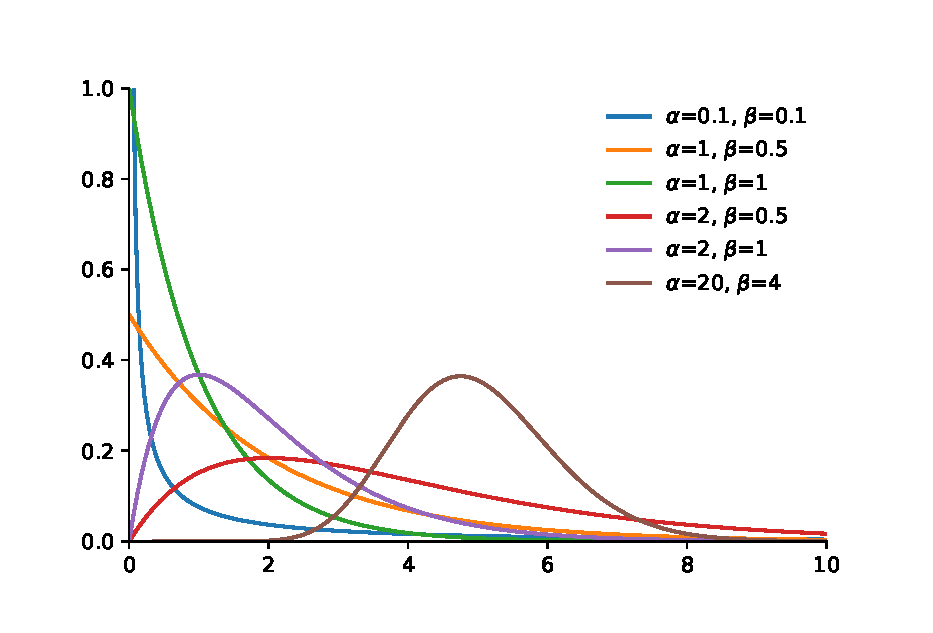
\includegraphics[width=0.8\textwidth]{ch3/gamma.eps}
    \caption{Función de densidad de probabilidad (pdf) de una distribución Gamma para diferentes parámetros de forma $\alpha$ y tasa $\beta$.}
    \label{img:gamma}
\end{figure}

\subsection{Configuración de hiperparámetros del grafo temporal}
\label{sec:graph_hiperparameters}

El grafo temporal cuenta con dos hiperparámetros: $q$ y $\zeta$. El parámetro $q \in [0,1]$ define el soporte de los tópicos, utilizando aquellas palabras más probables que explican q\% de la distribución acumulada del tópico. Por otro lado, el hiperparámetro $\zeta\in[0,1]$ define el úmbral de corte, representa el punto operante de la cdf del grafo \textit{fully-connected}, permite definir el cuantil que se usará como úmbral para eliminar arcos con similitud menor a este.\\

En cuanto al parámetro $q$ un valor razonable podría estar entre $[0.8, 0.95]$, de esta manera se conserva el \textit{core} de palabras del tópico y se disminuye de manera significativa el tiempo de cómputo. Por otro lado, valores razonables de $\zeta$ podrían estar entre $[0.9, 0.99]$, de esta manera solo se conservarían aquellas relaciones con una alta similitud relativa, debido a que el umbral de corte no depende de la medida de similitud utilizada.

\section{Resumen metodología}
\label{sec:methodology_resume}

En la Figura \ref{img:scheme} se presenta un esquema que resume la metodología propuesta para el descubrimiento y seguimiento de tópicos en el tiempo. En primer lugar, se divide el corpus original en épocas y a cada época se le aplican las siguientes cinco etapas en forma secuencial: tokenización, procesamiento de caracteres, eliminación de \textit{stopwords}, filtro por vocabulario y filtro por frecuencia. Como producto del proceso anterior se obtiene un corpus listo para la aplicación de un modelo de tópicos. En segundo lugar, se aplica HDP de forma independiente sobre cada una de las épocas. Por último, una vez descubiertos los tópicos se procede a construir el grafo temporal, para esto es necesario computar la WMD entre los tópicos de épocas adyacentes. Finalmente, se podan los arcos cuya similitud es menor al cuantil $\zeta$ de la distribución acumulada del grafo \textit{fully-connected}.

\def\db[#1,#2,#3,#4,#5]#6{%
  \node[draw, cylinder, alias=cyl, shape border rotate=90, aspect=#3, %
  minimum height=#1, minimum width=#2, outer sep=-0.5, color=black] (#4) at #5 {};%
  \node at #5 {#6};%
}
\def\boxtext[#1,#2,#3,#4,#5]#6{
        \node[draw=black, rounded corners, minimum height=#1,minimum width=#2, text width=6em] (#4) at #5 {}; 
        \node[anchor=#3,inner sep=4pt,] at (#4.#3)  {#6};
}
\def\isaedge[#1,#2,#3,#4];{ 
  \draw[-triangle 60,color=black!20!black,#4,fill=white] (#1) -- #3
  (#2);  
}

\begin{figure}
\begin{tikzpicture}
\db[45,40,1.6,db1,(0,2.2)] {
    \scriptsize\begin{tabular}{l}
        Corpus\\
        Original
    \end{tabular}
};
\boxtext[220,120,north,p,(3.5,2.2)] {\textbf{Procesamiento}};
\isaedge[db1,p,,];
\boxtext[180,100,south,p0,(3.5,2)] {$1:T$};
\boxtext[15,20,north,p1,(3.5,4.6)] {\footnotesize Tokenización};
\boxtext[15,20,north,p2,(3.5,3.4)]{\footnotesize Caracteres};
\boxtext[15,20,north,p3,(3.5,2.2)]{\footnotesize Stopwords};
\boxtext[15,20,north,p4,(3.5,1.0)]{\footnotesize Vocabulario};
\boxtext[15,20,north,p5,(3.5,-0.2)]{\footnotesize Frecuencia};
\isaedge[p1,p2,,];
\isaedge[p2,p3,,];
\isaedge[p3,p4,,];
\isaedge[p4,p5,,];
\db[45,40,1.6,db2,(7,2.2)] {
    \scriptsize\begin{tabular}{l}
        Corpus\\
        Procesado
    \end{tabular}
};
\isaedge[p,db2,,];
\boxtext[50,50,north,hdp,(9.7,2.2)] { 
    \begin{tabular}{l}
        \textbf{Tópicos}\\
        HDP $1:T$
    \end{tabular}
};
\isaedge[db2,hdp,,];
\boxtext[80,100,north,g,(13.5,2.2)] {\textbf{Grafo Temporal}};
\isaedge[hdp,g,,];
\boxtext[15,40,north,g1,(13.5,2.6)]{\footnotesize WMD};
\boxtext[15,40,north,g2,(13.5,1.4)]{\footnotesize Prunning};
\isaedge[g1,g2,,];
\end{tikzpicture}
\caption{Esquema de la metodología de descubrimiento y evolución de tópicos.}
\label{img:scheme}
\end{figure}
